\documentclass[12pt, twoside]{article}
\usepackage[letterpaper, margin=1in, headsep=0.2in]{geometry}
\setlength{\headheight}{0.6in}
%\usepackage[english]{babel}
\usepackage[utf8]{inputenc}
\usepackage{microtype}
\usepackage{amsmath}
\usepackage{amssymb}
%\usepackage{amsfonts}
\usepackage{siunitx} %units in math. eg 20\milli\meter
\usepackage{yhmath} % for arcs, overparenth command
\usepackage{tikz} %graphics
\usetikzlibrary{quotes, angles}
\usepackage{graphicx} %consider setting \graphicspath{{images/}}
\usepackage{parskip} %no paragraph indent
\usepackage{enumitem}
\usepackage{multicol}
\usepackage{venndiagram}

\usepackage{fancyhdr}
\pagestyle{fancy}
\fancyhf{}
\renewcommand{\headrulewidth}{0pt} % disable the underline of the header
\raggedbottom
\hfuzz=2mm %suppresses overfull box warnings

\usepackage{hyperref}

\fancyhead[LE]{\thepage}
\fancyhead[RO]{\thepage \\ Name: \hspace{4cm} \,\\}
\fancyhead[LO]{BECA / Dr. Huson / Geometry\\*  Unit 1: Segments, length, and area\\* 11 Sept 2022}

\begin{document}

\subsubsection*{1.4 Homework: Segments}
\begin{enumerate}
\item Line segments that have the same length are $\rule{4cm}{0.15mm}$.

\item Two line segments or angles of equal measure are $\rule{4cm}{0.15mm}$. \bigskip

\item The vertical line segment $\overline{PQ}$ is plotted on the coordinate plane with $P(4,8)$ and $Q(4,2)$. 
\begin{multicols}{2}
    Find the length $PQ$. \\[0.5cm]
    Show the calculation, including the absolute value bars. Count on the grid as a check. (leave marks)
    \begin{flushright}
    \begin{tikzpicture}[scale=.635]
        \draw [help lines] (-1,-1) grid (9,9);
        \draw [thick, ->] (-1.2,0) -- (9.4,0) node [below right] {$x$};
        \draw [thick, ->] (0,-1.2)--(0,9.4) node [left] {$y$};
        \draw [-, thick] (4,8)--(4,2);
        \draw [fill] (4,8) circle [radius=0.05] node[above right]{$P(4,8)$};
        \draw [fill] (4,2) circle [radius=0.05] node[below right]{$Q(4,2)$};
    \end{tikzpicture}
    \end{flushright}
\end{multicols} 

\item The horizontal line segment $\overline{RS}$ is plotted on the coordinate plane with $R(1,3)$ and $S(5,3)$. 
\begin{multicols}{2}
    Find the length $RS$. \\[0.5cm]
    Show the calculation.
    \begin{flushright}
    \begin{tikzpicture}[scale=.635]
        %\draw [help lines] (-1,-1) grid (9,9);
        \draw [thick, ->] (-1.2,0) -- (9.4,0) node [below right] {$x$};
        \draw [thick, ->] (0,-1.2)--(0,6.4) node [left] {$y$};
        \draw [-, thick] (1,3)--(5,3);
        \draw [fill] (1,3) circle [radius=0.05] node[below]{$R(1,3)$};
        \draw [fill] (5,3) circle [radius=0.05] node[below right]{$S(5,3)$};
    \end{tikzpicture}
    \end{flushright}
\end{multicols} 


\newpage
\item Given $\triangle JKL$ with $\overline{JK} \cong \overline{KL}$. On the diagram mark the congruent line segments with tick marks.
  \begin{center}
  \begin{tikzpicture}[scale=0.5]
    \draw [thick](0,0)--(9,0)--(4,8)--(0,0);
    \draw [fill] (0,0) circle [radius=0.05] node[below]{$J$};
    \draw [fill] (9,0) circle [radius=0.05] node[below]{$K$};
    \draw [fill] (4,8) circle [radius=0.05] node[above right]{$L$};
  \end{tikzpicture}
  \end{center}

\item Given the rectangle $ABCD$ shown below.
  \begin{enumerate}
    \item Measure and mark the length and width of the rectangle in centimeters.
    \item Calculate the area of the rectangle in square centimeters. (show your work)
  \end{enumerate} \vspace{2cm}
  \begin{center}
  \begin{tikzpicture}
    \draw [-, thick] (0,0)--(9,0)--(9,3)--(0,3)--cycle;
    \draw [fill] (0,0) circle [radius=0.05] node[left]{$A$};
    \draw [fill] (9,0) circle [radius=0.05] node[right]{$B$};
    \draw [fill] (9,3) circle [radius=0.05] node[right]{$C$};
    \draw [fill] (0,3) circle [radius=0.05] node[left]{$D$};
  \end{tikzpicture}
  \end{center}


\newpage
\item Given $\overline{ABC}$, $AB=3.8$, and $BC=1.7$. Find ${AC}$. \par \bigskip
  \begin{tikzpicture}
    \draw [-, thick] (1,0)--(7,0);
    \draw [fill] (1,0) circle [radius=0.05] node[below]{$A$};
    \draw [fill] (5,0) circle [radius=0.05] node[below]{$B$};
    \draw [fill] (7,0) circle [radius=0.05] node[below]{$C$};
  \end{tikzpicture} \vspace{1cm}

\item Given $\overline{DEF}$, $DE=3 \frac{1}{3}$, and $EF=1$. Find ${DF}$. \par \bigskip
  \begin{tikzpicture}
    \draw [-, thick] (1,0)--(7,0);
    \draw [fill] (1,0) circle [radius=0.05] node[below]{$D$};
    \draw [fill] (5,0) circle [radius=0.05] node[below]{$E$};
    \draw [fill] (7,0) circle [radius=0.05] node[below]{$F$};
  \end{tikzpicture} \bigskip

\item Given $\overline{PQR}$, $PQ=x-2$, $QR=x$, $PR=10$. Find ${PQ}$.
\begin{flushright}
  \begin{tikzpicture}
    \draw [-, thick] (0,0)--(7,0);
    \draw [fill] (0,0) circle [radius=0.05] node[below]{$P$};
    \draw [fill] (3,0) circle [radius=0.05] node[below]{$Q$};
    \draw [fill] (7,0) circle [radius=0.05] node[below]{$R$};
  \end{tikzpicture}
\end{flushright} \vspace{1cm}
      
\end{enumerate}
\end{document}